

由于软件的运行性能和处理器的结构有着非常紧密的联系,所以本节首先介绍龙芯3号系列处理器的硬件体系特点,为后续章节的优化工作做出理论基础。

\subsection{龙芯3A处理器介绍}
龙芯3A是龙芯多核处理器系列的第一款产品,是一个配置为单节点4核的龙芯3号处理器,采用65nm工艺制造,最高工作主频为1GHz,主要特征如下:

\begin{itemize}
\item{}片内集成四个64位的四发射超标量GS464高性能处理器核;
\item{}每个处理器核包括2个全流水的64位双精度浮点乘加部件;
\item{}每个处理器核包含64KB数据Cache和64KB的指令Cache;
\item{}片内集成四核共享的4MB二级Cache;
\item{}通过目录协议维护多核及I/O DMA访问的Cache一致性;
\item{}片内集成2个64位400MHz的DDR2/3控制器;
\item{}片内集成2个16位800MHz的HyperTransport控制器;
\item{}每个16位的HT端口拆分成两个8路的HT端口使用;
\item{}片内集成32位100MHz PCIX/66MHz PCI;
\item{}一个LPC、两个UART、1个SPI、16路GPIO接口;
\item{}采用128位AXI接口的交叉开关网络。
\end{itemize}

\begin{figure}[H] 
  \centering
  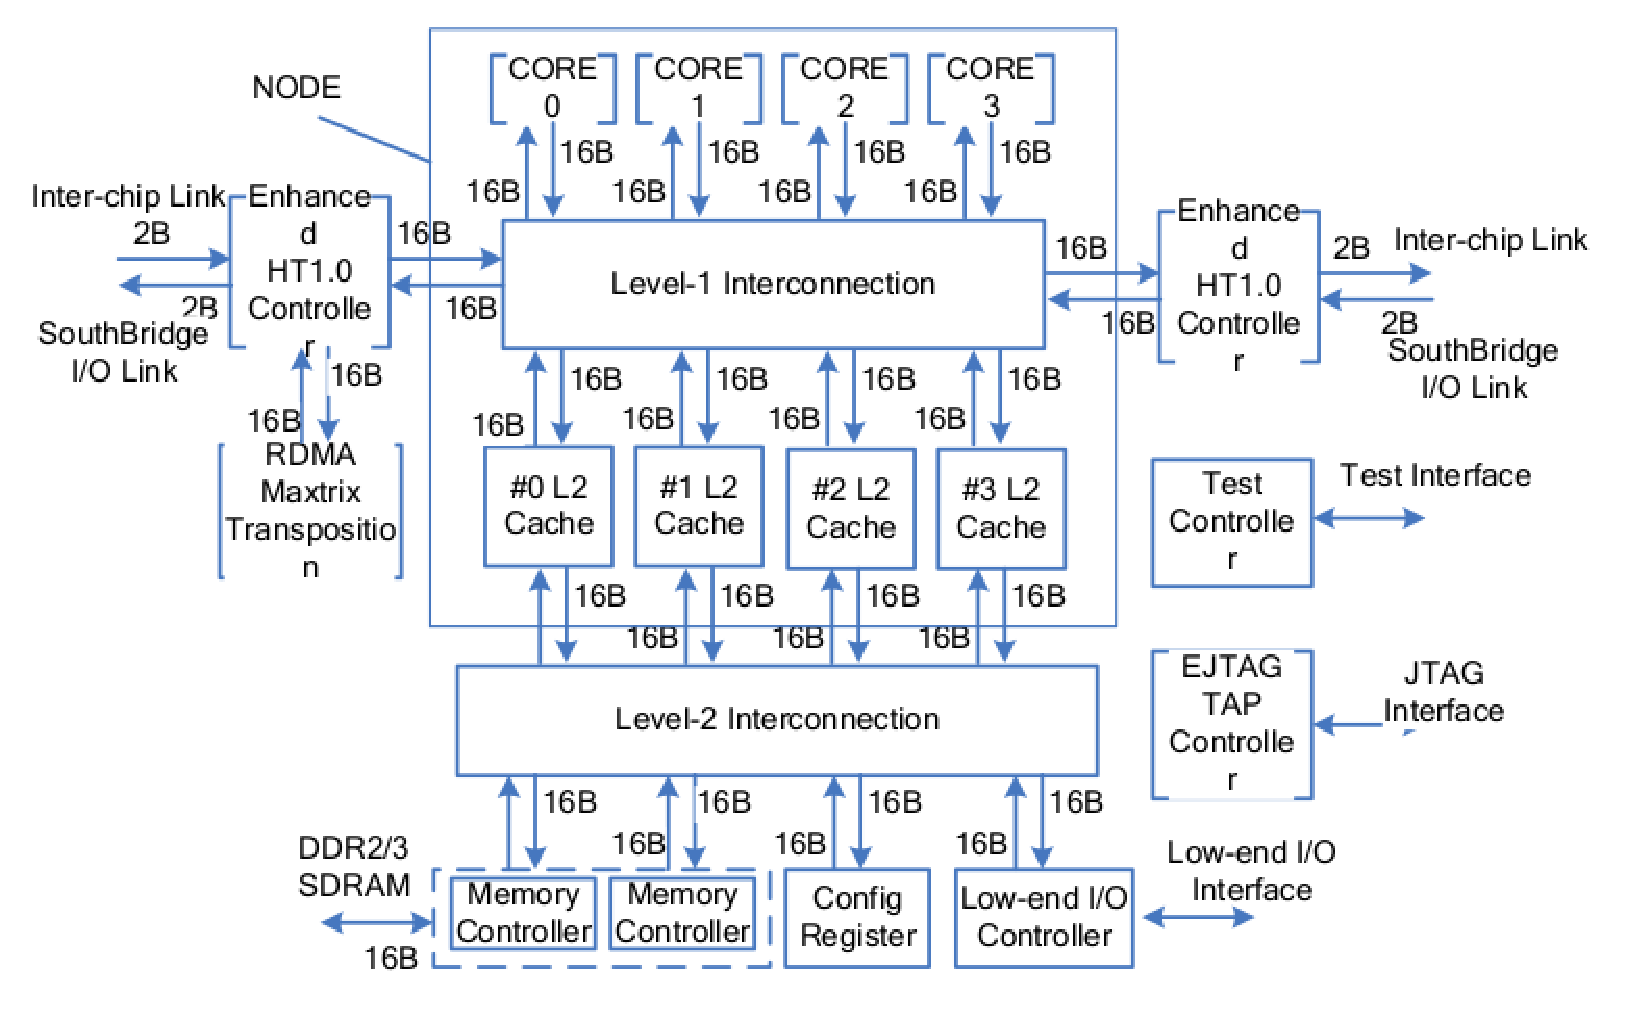
\includegraphics[width=10cm,height=6cm]{figures/chap02/Loongson3A}
  \caption{龙芯3A芯片结构}
  \label{fig:loongson3a}
\end{figure}

龙芯3A号芯片整体架构基于两级互连实现,结构如图\ref{fig:loongson3a}所示。由于四核龙芯3A在单芯片只包含一个节点,不用跟其他结点互连,因此第一层互连采用6x6的交叉开关,用于连接四个CPU(作为主设备)、四个二级Cache 模块(作为从设备)、以及两个IO端口(每个端口使用一个Master和一个Slave)。X1连接的每个IO端口连接一个16位的HT控制器,每个16位的HT端口还可以作为两个8位的HT端口使用。 HT控制器通过一个DMA控制器和X1相连, DMA控制器负责IO的DMA控制并负责片间一致性的维护。龙芯3号的DMA控制器还可以通过配置实现预取和矩阵转置\cite{Loongson3A-Manual}。


\subsection{龙芯3号平台Radeon显卡介绍}

在龙芯3号系列处理是平台上常用到的显卡设备就是Radeon系列显卡,本文的Mesa3D硬件加速相关的优化都是基于Radeon系列显卡实现的,所以这里对该系列显卡做简单的介绍。

\subsubsection{Radeon显卡命令处理机制}
Radeon显卡提供驱动使用命令流(Command Stream)的形式进行对显卡编程:驱动程序将需要对显卡进行配置的一连串命令写入命令缓冲区,写完之后进入让出处理器,显卡按照命令写入的顺序执行这些命令,执行完成后触发中断通知驱动。具体来说就是CPU将这些命令放入一个称为命令环的环形缓冲区中,命令环是GTT内存中分出来的一片内存,驱动程序往命令环中填充命令,填充完后通知GPU已经写入命令,接着GPU的命令处理器CP(Command Processor)接收并解析驱动程序发送过来的命令流,将解析后的数据传输给图形控制器的其他模块,包括3D图形处理器、2D图形处理器、视频处理器。

\begin{figure}[H] 
  \centering
  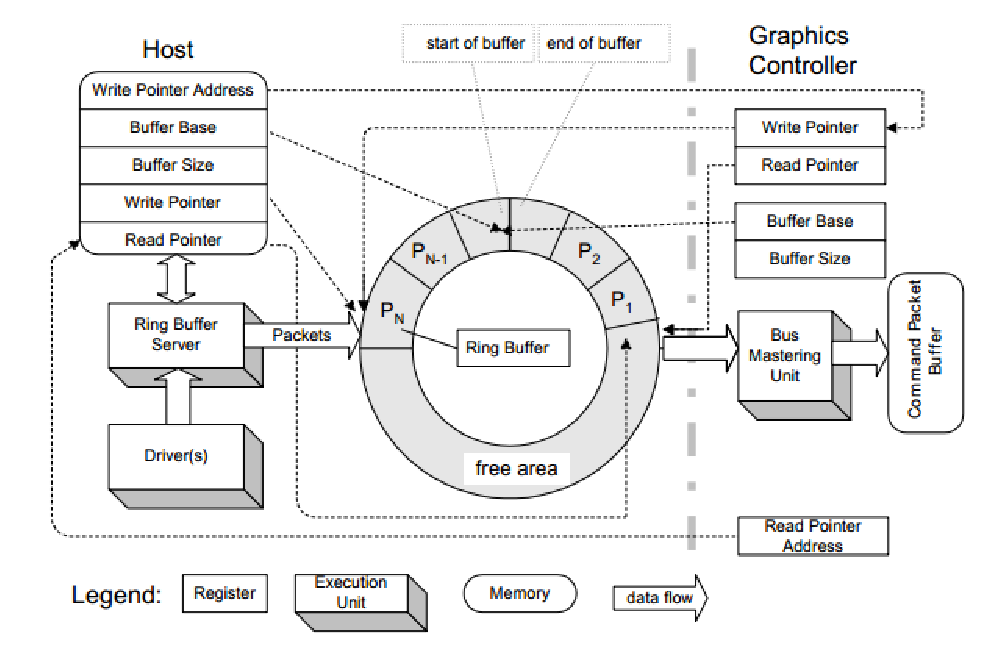
\includegraphics[width=10cm,height=6cm]{figures/chap02/CommandBuffer}
  \caption{Radeon显卡命令处理机制}
  \label{fig:CommandBuffer}
\end{figure}

\subsubsection{Radeon显卡3D图形渲染管线}

Radeon系列显卡通过内置的3D图形流水线帮助实现图形渲染的硬件加速,这里以Radeon R600显卡为例介绍其内部的图形流水线结构。

\begin{figure}[H] 
  \centering
  \includegraphics[width=9cm,height=10cm]{figures/chap02/R600-Pipeline}
  \caption{R600图形渲染管线}
  \label{fig:R600-Pipeline}
\end{figure}

如图\ref{fig:R600-Pipeline}所示,输入数据大体上按照“顶点处理”、“图元组装”、“光栅化”、“片段处理”、“输出”的过程流经图形硬件。这些阶段几乎完全覆盖了前面图\ref{fig:OpenGL-Pipeline}里面的渲染过程,更加详细信息可查阅参考文献Radeon R6xx/R7xx Acceleration\cite{Radeon-Manual}。
